\documentclass{../lab}

\labacronym{BMC}
\labtitle{Brownian Motion in Cells}

%\newcommand{\SimulatingBrownianMotion}{http://experimentationlab.berkeley.edu/node/83}
%\newcommand{\ExperimentalProcedures}{http://experimentationlab.berkeley.edu/node/84}
%\newcommand{\BMCPreLabandEvaluation}{http://experimentationlab.berkeley.edu/BMCPreLab}
%\newcommand{\movieanimationofkinesin}{https://vimeo.com/157524451}
%\newcommand{\}{http://physics111.lib.berkeley.edu/Physics111/Reprints/BMC/Zeiss-Microscope_46-0015_e.pdf}

\begin{document}

\maketitle

\tableofcontents

\section{Brownian Motion in Cells Description (BMC)}

\begin{enumerate}
    \item \textbf{Note that there is NO eating or drinking in the 111-Lab anywhere, except in rooms 282 \& 286 LeConte on the bench with the BLUE stripe around it.} Thank You - the Staff.
\end{enumerate}

This is a Biophysics experiment. Small particles suspended in a liquid wiggle around furiously. It took the mind of Albert Einstein to change this from a curious observation to an important evidence for the then controversial atomic theory of matter. Einstein realized that the random motions (called Brownian motion) could be explained by the molecular kinetic theory. In 1905, Einstein published a paper that predicted a relationship between the mean-squared magnitude of Brownian excursions and the size of molecules. Now all that remained was to do the experiment. Jean Perrin won the Nobel Prize in 1926 for his work confirming Einstein's hypothesis.

Perrin's experimental confirmation of Einstein's equation was an important piece of evidence to help settle a debate about the nature of matter that had begun nearly 2000 years earlier in the time of Democritus and Anaxagoras. Since then, a thorough understanding of Brownian motion has become essential for diverse fields ranging from polymer physics to biophysics, aerodynamics to statistical mechanics, and even stock option pricing.

Thank you to Professor Jan T. Liphardt for his ideas for this experiment. This experiment has also been made possible by the generous donations from the Stanford Research Systems to the University of California at Berkeley Physics 111-Laboratory. Thank you very much.

\begin{enumerate}
    \item Pre-requisites: Microsoft Windows, Matlab knowledge

    \item Days Allotted for the Experiment: 8
\end{enumerate}

\textbf{To get a copy of the Full Lab Write-up click on each link below and print separately}

\begin{enumerate}
    \item \textbf{Brownian Motion in Cells} (current page)
    
    \item \href{http://experimentationlab.berkeley.edu/node/83}{\textbf{Simulating Brownian Motion}}
    
    \item \href{http://experimentationlab.berkeley.edu/node/84}{\textbf{Experimental Procedures}}
    
    \item \href{http://experimentationlab.berkeley.edu/node/85}{\textbf{BMC Software}}
\end{enumerate}

This lab will be graded 30\% on theory, 30\% on technique, and 40\% on analysis. For more information, see the \href{\AdvancedLabSyllabus}{\textbf{Advanced Lab Syllabus}}.

Comments: E-mail \href{\MailDonOrlando}{\textbf{Don Orlando}}

\section{The Brownian Motion in Cells Experiment Photos}

\begin{figure}[H]
\minipage{0.32\textwidth}
  \href{http://experimentationlab.berkeley.edu/sites/default/files/upimages/BMC\%20Supplies\%20on\%20Shelves_2541.JPG}{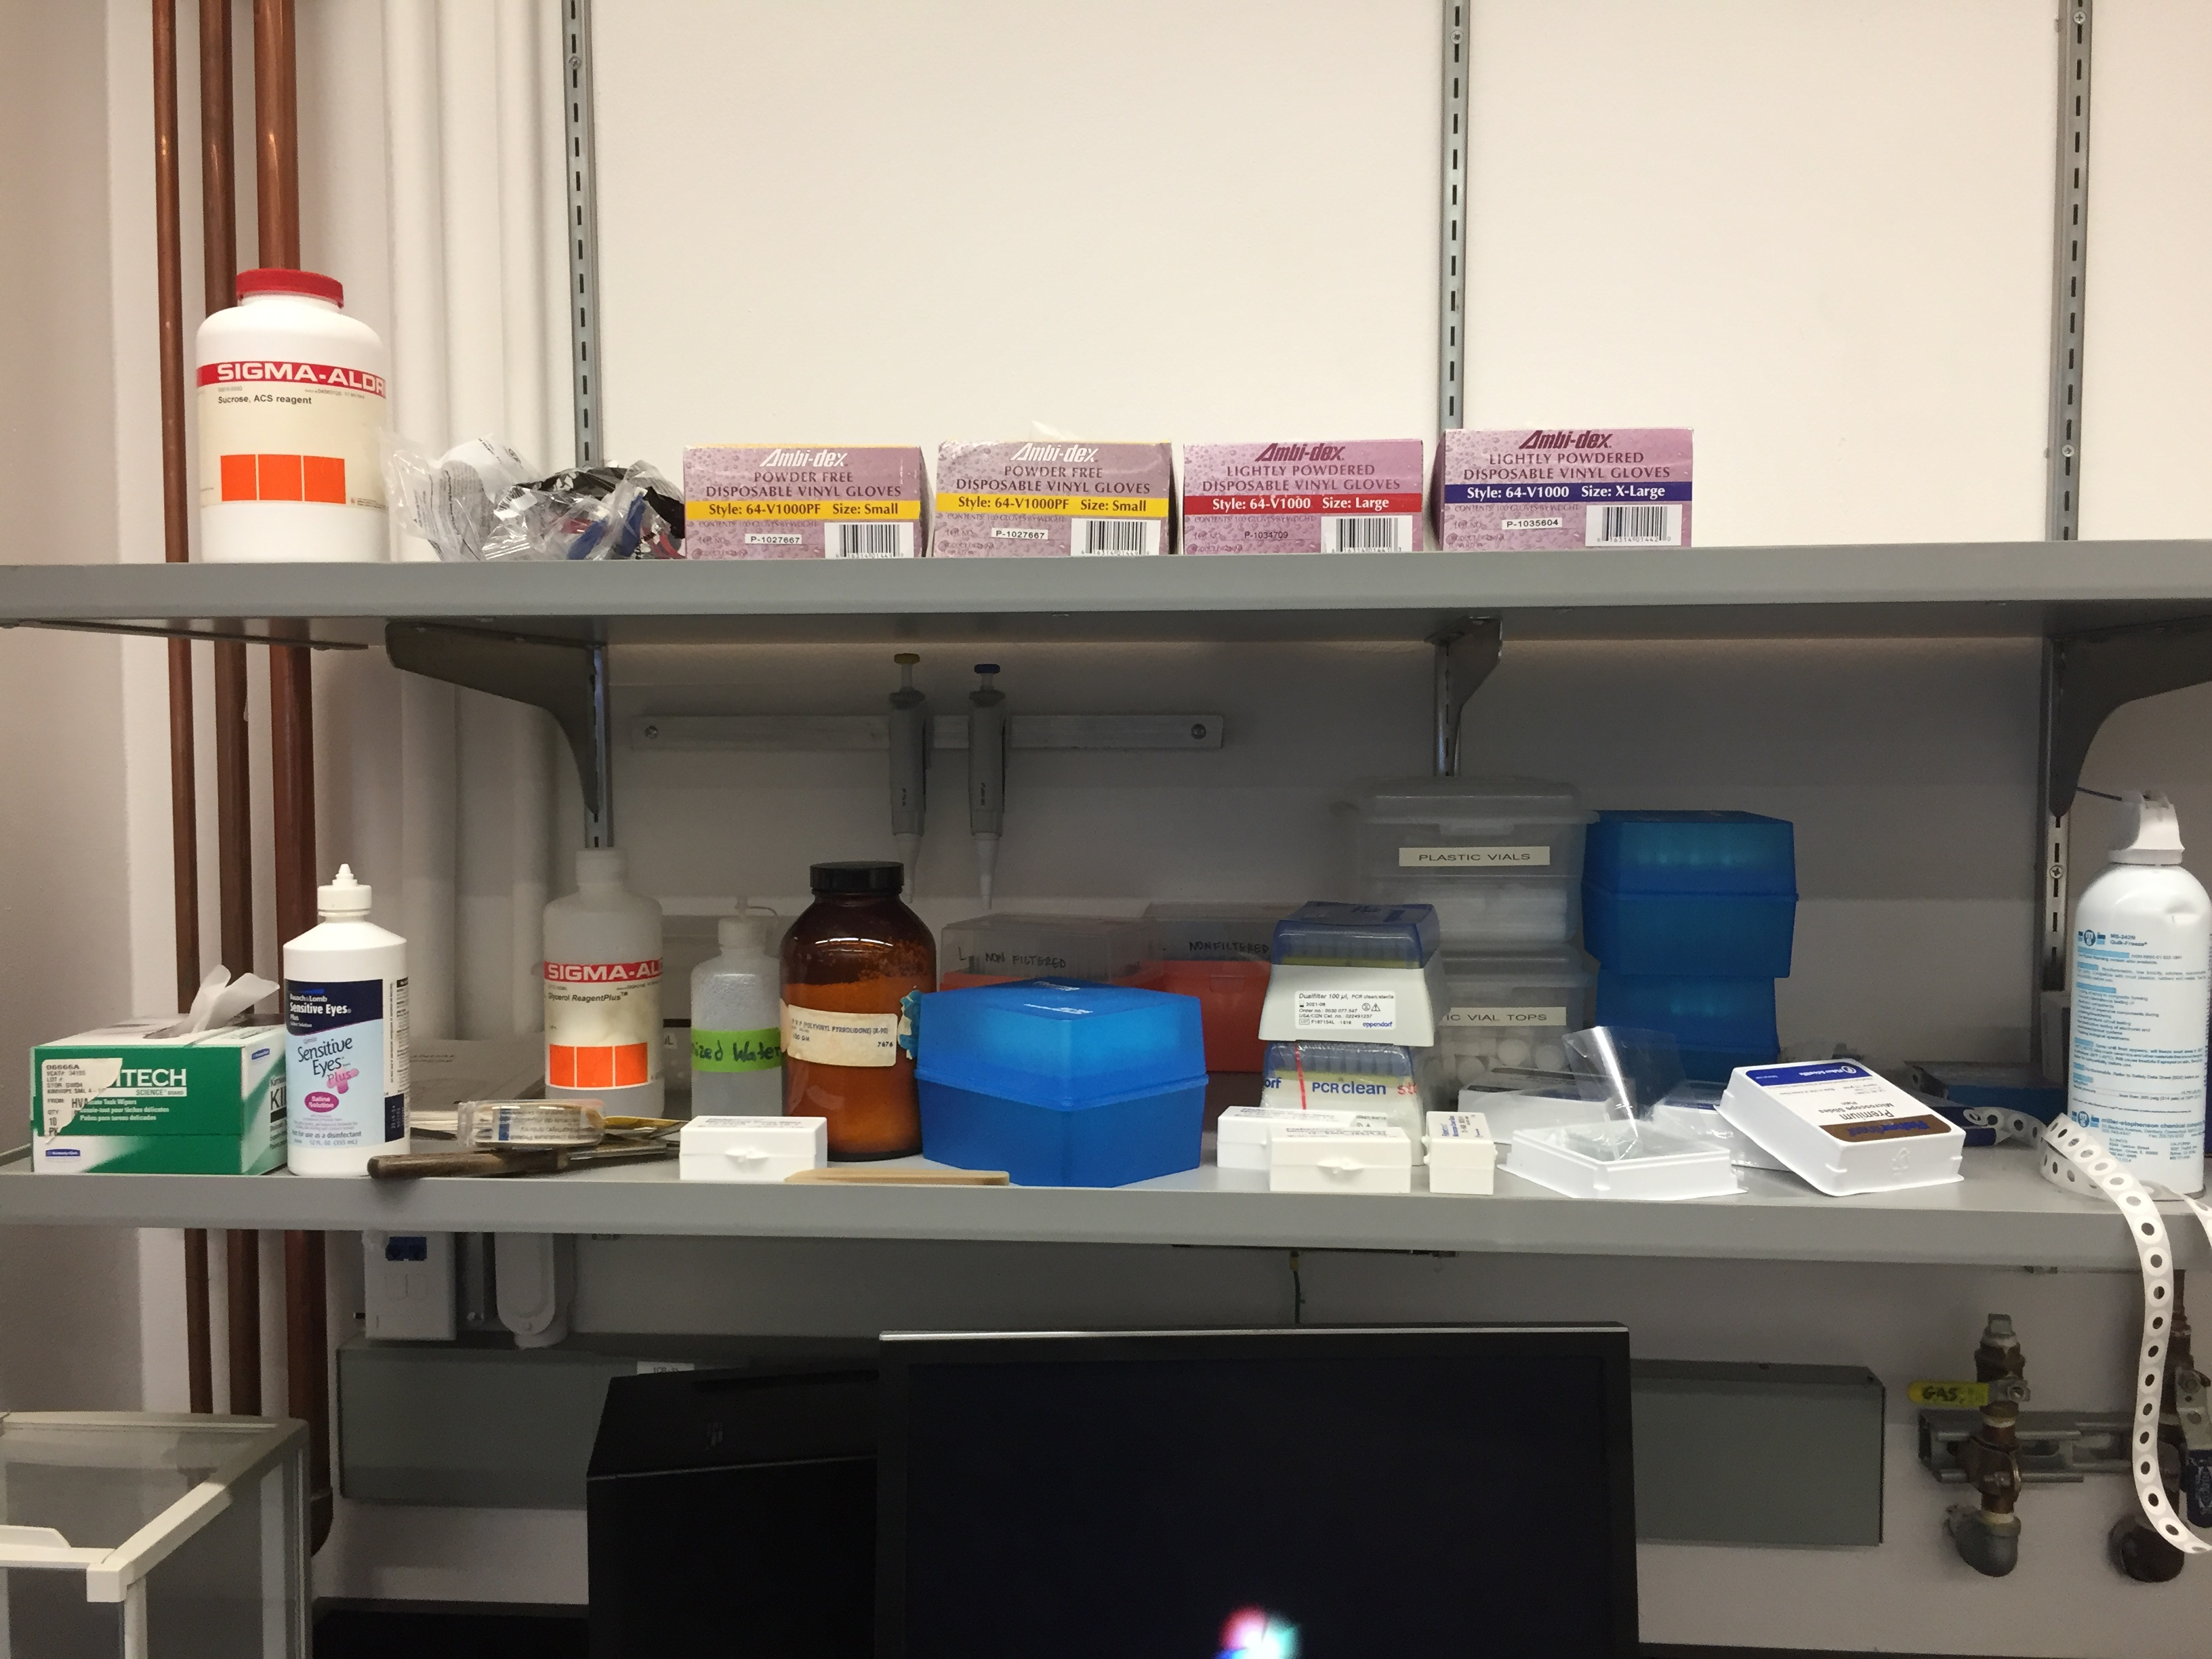
\includegraphics[width=\linewidth,keepaspectratio]{images/IMG_2541.JPG}}
  \caption{Supplies on shelves \\ \href{http://experimentationlab.berkeley.edu/sites/default/files/upimages/BMC\%20Supplies\%20on\%20Shelves_2541.JPG}{Click here to see larger picture}}
  \label{fig:Supplies}
\endminipage\hfill
\minipage{0.32\textwidth}
  \href{http://experimentationlab.berkeley.edu/sites/default/files/upimages/2_Legend-Microscope_2540.JPG}{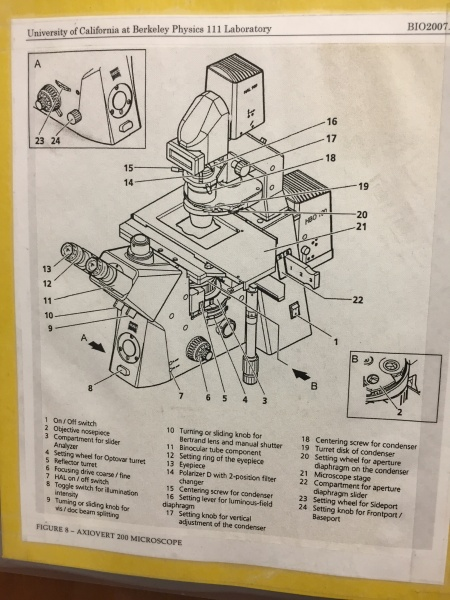
\includegraphics[width=\linewidth,keepaspectratio]{images/2_Legend-Microscope_2540.JPG}}
  \caption{Microscope apparatus legend \\
  \href{http://experimentationlab.berkeley.edu/sites/default/files/upimages/2_Legend-Microscope_2540.JPG}{Click here to see larger picture}}
  \label{fig:MicroscopeLegend}
\endminipage\hfill
\minipage{0.32\textwidth}
  \href{http://experimentationlab.berkeley.edu/sites/default/files/upimages/1_Microscope_2539.JPG}{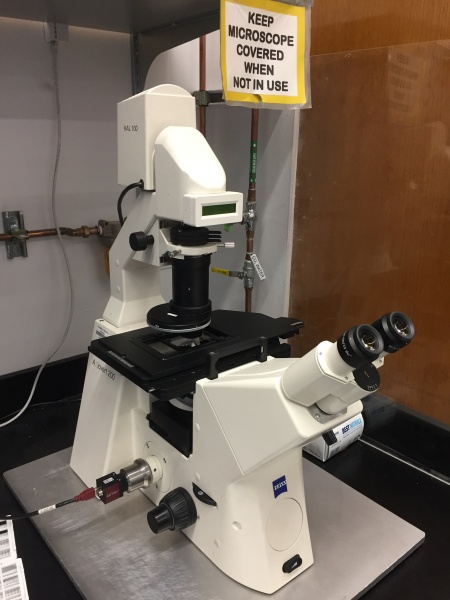
\includegraphics[width=\linewidth,keepaspectratio]{images/1_Microscope_2539.JPG}}
  \caption{Microscope front view\\ \href{http://experimentationlab.berkeley.edu/sites/default/files/upimages/1_Microscope_2539.JPG}{Click here to see larger picture}}\label{fig:Microscope}
\endminipage
\end{figure}

\begin{figure}[H]
\minipage{0.32\textwidth}
  \href{http://experimentationlab.berkeley.edu/sites/default/files/upimages/Slide-on-Microscope_2544.JPG}{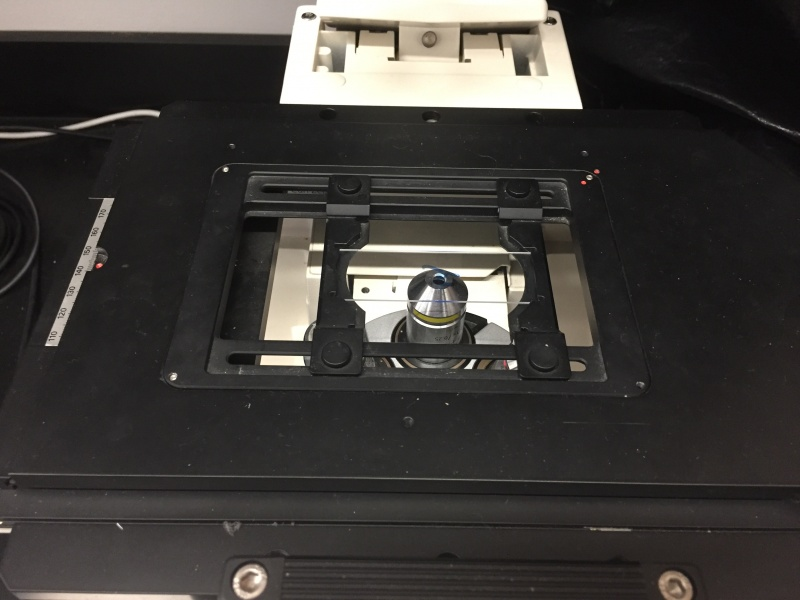
\includegraphics[width=\linewidth,keepaspectratio]{images/Slide-on-Microscope_2544.JPG}}
  \caption{Slide on microscope\\ \href{http://experimentationlab.berkeley.edu/sites/default/files/upimages/Slide-on-Microscope_2544.JPG}{Click here to see larger picture}}
  \label{fig:MicroscopeSlide}
\endminipage\hfill
\minipage{0.32\textwidth}
  \href{http://experimentationlab.berkeley.edu/sites/default/files/upimages/1_Tilt-Microscope_2542.JPG}{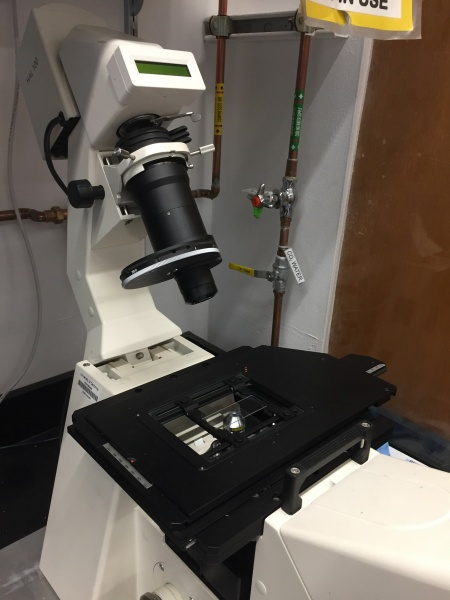
\includegraphics[width=\linewidth,keepaspectratio]{images/1_Tilt-Microscope_2542.JPG}}
  \caption{Micrscope tilted back \\
  \href{http://experimentationlab.berkeley.edu/sites/default/files/upimages/1_Tilt-Microscope_2542.JPG}{Click here to see larger picture}}
  \label{fig:TiltMicroscope}
\endminipage\hfill
\minipage{0.32\textwidth}
  \href{http://experimentationlab.berkeley.edu/sites/default/files/upimages/6_eye-wear-face.jpg}{
\includegraphics[width=\linewidth,keepaspectratio]{images/6_eye-wear-face_small.jpg}}
  \caption{Wear your safety glasses! \\ \href{http://experimentationlab.berkeley.edu/sites/default/files/upimages/6_eye-wear-face.jpg}{Click here to see larger picture}}\label{fig:EyeWear}
\endminipage
\end{figure}

\section{Before the 1st Day of Lab}

\textbf{Complete the following before your scheduled start date of the experiment:}

\begin{enumerate}
    \item \emph{\textbf{Note: In order to view the private Youtube videos hosted by the university, you must be signed into your berkeley.edu Google account.}} \\
    View the \href{http://youtu.be/XJ6YBTL6euc}{\textbf{Brownian Motion in Cells Video}}

    \item \emph{Checkpoints are examination points where you must STOP and get a GSI or professor to verify your understanding and/or verify proper experimental setup. You cannot skip the checkpoints, as there is a \href{http://experimentationlab.berkeley.edu/bmccheckpoints}{\textbf{sign off sheet}} that must be turned in with your lab report. If you fail to pass the checkpoints, you fail the lab.}

    \item Complete the \href{http://experimentationlab.berkeley.edu/BMCPreLab}{\textbf{BMC Pre Lab and Evaluation}} sheets. Print, fill it out, then turn it in filled out with your answers. The Pre-Lab must be printed separately. Discuss the experiment and pre-lab questions with any faculty member or GSI and get it signed off by that faculty member or GSI. Turn in the signed pre-lab sheet with your lab report.

    \item Decide which combinations of bead size, viscosity, and solute you will use in  \hyperref[sec:InvestigationI]{Investigation I}.

    \item Before you make observations with the microscope, you will \href{http://experimentationlab.berkeley.edu/node/83}{\textbf{Run the Simulating Brownian Motion}} in Matlab exercise and be prepared to discuss the ways of visualizing and analyzing particle motion.  A sample simulation script is provided. Show your simulation results and the answers to the following questions to a GSI or professor before you start. Copy the folder ``Brownian Motion Software'' on the ``C'' drive to your ``My Documents'' folder and run it there.

    \item Last day of the experiment please fill out the \href{\ExperimentEvaluation}{\textbf{Experiment Evaluation}}
\end{enumerate}

Run the ``Brownian Motion in Matlab'' exercise.

\begin{enumerate}
    \item \textbf{NOTE: To close the program windows just X out the camera window, it will close ALL windows.}
\end{enumerate}

\textbf{Suggested Reading:}

\begin{enumerate}
    \item A. Einstein, ``\href{http://physics111.lib.berkeley.edu/Physics111/Reprints/BMC/Einstein\_Diffusion1905.pdf}{\textbf{On the Motion of Small Particles Suspended in Liquids at Rest Required by the Molecular-Kinetic Theory of Heat}}'', Annalen der Physik (1905). This is Einstein’s seminal Brownian motion paper. The derivations are a little hard to follow but it is a must read \& study to really understand the lab.

    \item E. Frey and K. Kroy, ``\href{http://physics111.lib.berkeley.edu/Physics111/Reprints/BMC/Brownian\%20Motion\%20-\%20Frey.pdf}{\textbf{Brownian motion: a paradigm of soft matter and biological physics}}'', Ann. Phys. (2005). Published on the 100th anniversary of Einstein’s paper, this reference chronicles the history of Brownian motion from 1905 to the present. The first 15 pages are helpful in understanding both the concepts and the derivations. The latter parts more apply to biological things and become less helpful as you get deeper into the paper, but you can skim by section and still find some good information. (See Sections 1-4)

    \item R. Newburgh, J. Peidle, and W. Rueckner, ``\href{http://physics111.lib.berkeley.edu/Physics111/Reprints/BMC/Newburgh-Einstein-Perrin1905_Revisited.pdf}{\textbf{Einstein, Perrin, and the reality of atoms: 1905 revisited}}'', Am. J. Phys. (2006). A modern replication of Perrin's experiment. This paper is a must read and has an easy to follow derivation which skips over some of the more laborious details.

    \item A great \href{http://www.physics.nyu.edu/grierlab/methods/methods.html}{\textbf{Primer on Particle Tracking, Data Analysis, and Diffusion}}.

    \item \href{\LabReprints}{\textbf{Physics 111-Lab Library site}}
\end{enumerate}

 More \hyperref[sec:References]{References} 

You should keep a laboratory notebook. The notebook should contain a detailed record of everything that was done and how/why it was done, as well as all of the data and analysis, also with plenty of how/why entries. This will aid you when you write your report.

\section{Objectives}

\begin{itemize}
    \item Learn how to use a microscope (focus on an image, achieve Kohler illumination, prepare slides)

    \item Use image analysis software to track particles

    \item Learn about MATLAB's statistics and simulation applications

    \item Witness the wondrous jiggling of tiny particles

    \item Learn about the mechanics of intracellular transport
\end{itemize}

\textbf{In the first part of this lab}, you will replicate Perrin's work with modern equipment. You will track the motion of synthetic beads suspended in liquids of various viscosities on a research-grade inverted microscope. A CCD camera (Guppy F038C NIR Color) will transfer images of the beads to a computer for automated particle tracking and analysis. You will explore the use of algorithms to improve the identification and tracking of particles as well as analyze the effects of particle size, viscosity of the solution, and molecular weight of the dissolved solute on the motion of the beads. You will use Matlab to estimate the positions of the particles and analyze the data to see if it conforms to Einstein's model. No programming is required; however, facility with computers is essential.

\textbf{In the second part of this lab} you will investigate the motion of vesicles inside living cells. Intracellular transport is accomplished either by Brownian motion or by directed transport by molecular motors that pull vesicles along cytoskeletal tracks running throughout the cell. After some initial observation of internal transport in onion cells, your task will be to choose a research question and carry out an investigation of your own design using the techniques you have learned in this lab.

Techniques developed and introduced in this lab include bright-field and dark-field microscopy, pipetting, image data acquisition, theory and software design for image filtering and particle tracking in C\#, simulations in Matlab, and data analysis in Matlab or Excel. Previous programming experience is not required.

\section{Introduction}

\subsection{Brownian Motion}

If you have ever looked at an aqueous sample through a microscope, you have probably noticed that every small particle you see wiggles about continuously. Robert Brown, a British botanist, was not the first person to observe these motions, but perhaps the first person to recognize the significance of this observation. Experiments quickly established the basic features of these movements. Among other things, the magnitude of the fluctuations depended on the size of the particle, and there was no difference between ``live'' objects, such as plant pollen, and things such as rock dust. Apparently, finely crushed pieces of an Egyptian mummy also displayed these fluctuations.

Brown noted: \emph{[The movements] arose neither from currents in the fluid, nor from its gradual evaporation, but belonged to the particle itself.}

This effect may have remained a curiosity had it not been for A. Einstein and M. Smoluchowski. They realized that these particle movements made perfect sense in the context of the then developing kinetic theory of fluids. If matter is composed of atoms that collide frequently with other atoms, they reasoned, then even relatively large objects such as pollen grains would exhibit random movements. This last sentence contains the ingredients for several Nobel prizes!

Indeed, Einstein's interpretation of Brownian motion as the outcome of continuous bombardment by atoms immediately suggested a direct test of the atomic theory of matter. J. Perrin received the 1926 Nobel Prize for validating Einstein's predictions, thus confirming the atomic theory of matter.

Since then, the field has exploded; a thorough understanding of Brownian motion is essential for everything from polymer physics to biophysics, aerodynamics, and statistical mechanics. One of the aims of this lab is to directly reproduce the experiments of J. Perrin that led to his Nobel Prize. A translation of the key work is included in the reprint folder. Have a look -- he used latex spheres, and we will use polystyrene spheres; otherwise the experiments will be identical. In addition to reproducing Perrin's results, you will probe further by looking at the effect of varying solvent molecule size.

\subsection{Intracellular Transport}

The second part of this experiment consists of observing the motion of particles inside a living cell. Cells transport food, waste, information, etc. in membrane-bound vesicles, which are visible under a light microscope. An old-fashioned view of a cell was that it is a ``bag of water'' containing various enzymes in which matter is transported passively by diffusion. Though diffusion is an important mechanism, it is too slow and random for long distance transport and directing materials where they are most needed, especially in larger cells. It is now understood that cells have highly developed and intricate mechanisms for directed transport of materials.

\begin{figure}[h]
\begin{minipage}{0.32\linewidth}
\centering
\href{http://experimentationlab.berkeley.edu/sites/default/files/images/250px-BMC_Cytoskeleton.jpg}{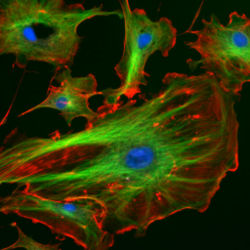
\includegraphics[width=\linewidth]{images/250px-BMC_Cytoskeleton.jpg}}
    \caption{The eukaryotic cytoskeleton. Actin filaments are shown in red, microtubules in green, and the nuclei are in blue.}
    \label{fig:250px-BMC_Cytoskeleton}
    \end{minipage}\hfill
\begin{minipage}{0.32\linewidth}
    \centering
    \href{http://experimentationlab.berkeley.edu/sites/default/files/images/Myosin.gif}{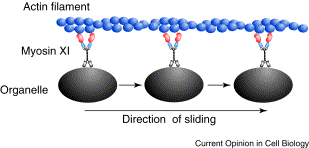
\includegraphics[width=\linewidth,keepaspectratio]{images/Myosin.png}} \\
    \caption{Cartoon of myosin motors pulling organelles along an actin filament.}
\end{minipage}\hfill
\begin{minipage}{0.32\linewidth}
    \centering
    \href{http://experimentationlab.berkeley.edu/sites/default/files/images/196px-Kinesin.jpg}{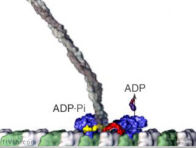
\includegraphics[width=\linewidth,keepaspectratio]{images/196px-Kinesin.jpg}} \\
    \caption{Binding of kinesin motor to microtubule.}
\end{minipage} 
\end{figure}

Most motions within and of cells involve two components, a cytoskeletal fiber that serves as a track, and a \href{http://physics111.lib.berkeley.edu/Physics111/Reprints/OTZ/biowikipedia.pdf}{\textbf{motor protein}} that does the work. The motor molecule uses energy from the hydrolysis of one ATP molecule to bind to the fiber, bend to pull itself along the fiber, and release, all of which constitutes one ``step''. For an animation of this stepping process, see this \href{http://experimentationlab.berkeley.edu/sites/default/files/Kinesin_Motion.mp4}{\textbf{movie animation}} from the Vale lab web site at UC San Francisco. One can divide cellular motility mechanisms into two classes based on the cytoskeletal fibers involved. Microtubule-based mechanisms involve dynein or kinesin motors pulling on microtubules made of the protein tubulin. Actin-based mechanisms involve myosin motors pulling on actin fibers, also called microfibers.

Virtually all cell types exhibit directed intracellular transport, but some cell types are particularly suitable for transport studies. Fish-scale pigment cells work well, since a large fraction of the cargoes that are transported are pigmented and thus easy to observe – the disadvantage is that you would need to bring a living fish into lab as a source of these cells. For convenience, we will use epidermal cells from onion bulbs that you can easily acquire in a grocery store. With some care, a single layer of cells can be peeled off from an inner section of the onion bulb and mounted flat on a slide.

\begin{figure}
\begin{minipage}[t]{.475\linewidth}
    \centering
    \href{http://experimentationlab.berkeley.edu/sites/default/files/images/250px-Image005.png}{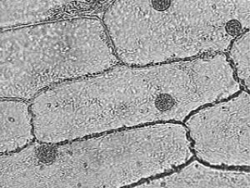
\includegraphics[width=\linewidth,keepaspectratio]{images/250px-Image005.png}} \\
    \caption{Onion cells in bright-field illumination. Round object in each cell is the nucleus.}
\end{minipage}\hfill
\begin{minipage}[t]{.475\linewidth}
    \centering
    \href{http://experimentationlab.berkeley.edu/sites/default/files/images/Image003.png}{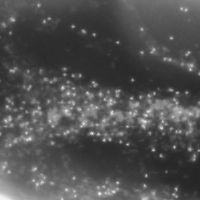
\includegraphics[width=\linewidth,keepaspectratio]{images/Image003.png}} \\
    \caption{Vesicles in the cytoplasm of a plant cell, as seen in dark-field.}
\end{minipage} 
\end{figure}

In this experiment, we will be viewing the movement of vesicles within the cytoplasm of onion epidermal cells, shown above as they appear in bright-field and dark-field microscopy. The layers you see in an onion bulb develop into leaves when it sprouts. Both sides of the leaf are covered with an epidermis consisting of brick-shaped cells, each with a cell wall and cell membrane on the outside. Most of the interior of the cell is filled with a clear fluid \href{http://physics111.lib.berkeley.edu/Physics111/Reprints/OTZ/biowikipedia.pdf}{\textbf{vacuole}} that functions in storage and in maintenance of hydrostatic pressure essential to the stiffness of the plant (the difference between crisp lettuce and wilted lettuce). The \href{http://physics111.lib.berkeley.edu/Physics111/Reprints/OTZ/biowikipedia.pdf}{\textbf{cytoplasm}}, containing all of the other cell contents, occurs in a thin layer between the cell membrane and the vacuole, and in thin extensions through the vacuole called transvacuolar strands. It is within the cytoplasm that you will be observing directed transport of vesicles by an actin-based mechanism. These vesicles are spherical or rod-shaped organelles such as mitochondria, spherosomes, and \href{http://physics111.lib.berkeley.edu/Physics111/Reprints/OTZ/biowikipedia.pdf}{\textbf{peroxisomes}} ranging in size from 0.5 to 3 microns. The diagram of an onion cell below shows the location of the cell wall, cytoplasm and vesicles in a typical cell; you will not be able to see much of the endoplasmic reticulum or the vacuole depicted because of their transparency. Under the microscope, you will notice the vesicles are located just along the edges of the cell, or near the top and bottom surface if you focus up and down. When you see a narrow band of moving vesicles in the center of the cell, it is located in a transvacuolar strand, which may be a handy place to study motion.

\begin{figure}[h]
    \centering
    \href{http://experimentationlab.berkeley.edu/sites/default/files/images/500px-BMC_OnionStucture.gif}{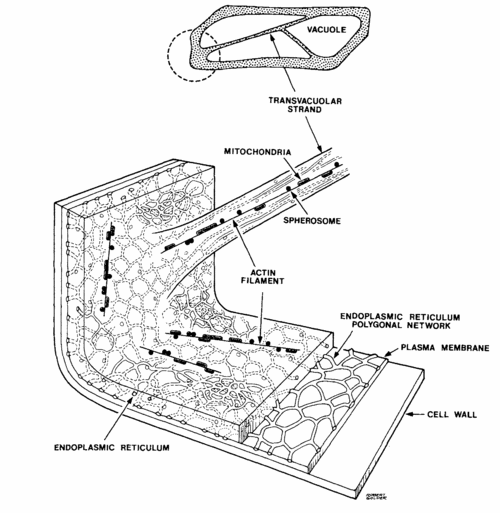
\includegraphics[width=0.8\linewidth]{images/500px-BMC_OnionStucture.png}}
    \caption{A 3D cross-section model of an onion epidermal cell, showing actin filaments and vesicles in the narrow bands of cytoplasm within the cell.}
    \label{fig:500px-BMC_OnionStucture}
\end{figure}

A 3D cross-section model of an onion epidermal cell, showing actin filaments and vesicles in the narrow bands of cytoplasm within the cell.In plant cells, vesicles are transported along actin fibers by myosin motor molecules. An actin filament is composed of two intertwined actin chains, about 7 nm in diameter. An actin fiber is considered structurally polar, having a (+) end and a (-) end, and most myosin motors move only towards the (+) end of the actin fiber. In order to reverse the direction of a vesicle's motion, the vesicle must grab on to another actin fiber oriented in the opposite direction. There are at least eighteen described classes of myosin, of which three, myosin VIII, XI, and XII are found in plant cells. Some myosin motors are processive, meaning that they remain bound to an actin fiber as they move step-by-step along it (analagous to this \href{http://experimentationlab.berkeley.edu/sites/default/files/Kinesin_Motion.mp4}{\textbf{movie animation of kinesin}}). Other myosins are non-processive, releasing from the actin fiber after each step. Myosin II found in muscle cells is non-processive, as illustrated in this \href{http://physics111.lib.berkeley.edu/Physics111/Reprints/OTZ/actinmyosin.gif}{\textbf{gif animation}}.  In the muscle functional unit, there are many myosin motors acting together, so there are always some attached to the actin fiber. The myosin XI responsible for transport of plant cell vesicles is the fastest myosin known and is processive. It is not certain how many myosin molecules are attached to the surface of a vesicle or how many of those are active at one time in pulling the vesicle along an actin fiber.

In some plant cells and algal cells, a large-scale streaming motion of the cytoplasm is observed, logically called \href{http://physics111.lib.berkeley.edu/Physics111/Reprints/OTZ/biowikipedia.pdf}{\textbf{cytoplasmic streaming}}. This bulk flow is believed to be caused by myosin motors pulling the extensive endoplasmic reticulum along actin fibers lining the cell membrane. Many other vesicles are then dragged along with the endoplasmic reticulum. \href{http://experimentationlab.berkeley.edu/sites/default/files/Lodish_and_Berk_Figure_18-40.pdf}{\textbf{Lodish and Berk, et al.}} provide a detailed explanation of this process and a video of cytoplasmic streaming in the pond weed Elodea can be viewed \href{http://experimentationlab.berkeley.edu/sites/default/files/Cytoplasmic_Streaming_Elodea.mov}{\textbf{here}}.

In your observations of vesicles in onion epidermal cells, you should distinguish between the random Brownian motion of vesicles that are unattached from (or at least not actively moving along) actin filaments, the directed transport of vesicles by attached myosin motors, and possibly (though we are not sure this really happens in onions) bulk flow of vesicles in cytoplasmic streaming.

\subsection{Supplies Used in this experiment}

\begin{enumerate}
    \item 0.47 $\mu$m Primary Blue \# DS02B (High density Sample)

    \item 1.0 $\mu$m PolyStyrene \# PS04N

    \item 6.0 $\mu$m P(S/2\%DVB) \# PS06N

    \item 10.0 $\mu$m P(S/2\%DVB) PolyStyrene \# PS07N

    \item Saline solution (contact lens solution)

    \item One fresh\textbf{ Onion} that you purchase

    \item 3'' x 1'' Microscope slides

    \item Coverslips

    \item Glycerol (as a solvent)

    \item polyvinylpyrrolidone (PVP) (As a solvent)

    \item Deionized water

    \item Micropipettes (10 - 100 $\mu l$, 100 - 1000 $\mu l$) and pipette tips

    \item Plastic vials with lids to mix solutions

\end{enumerate}

Description: Many proteins may be easily and stably absorbed to hydrophobic, non-functionalized microspheres. Divinylbenzene (DVB) confers additional solvent and heat resistance to the crosslinked spheres. PS and P(S/DVB) microspheres are available in four standard amounts. \href{http://physics111.lib.berkeley.edu/Physics111/Reprints/BMC/Colloid\%20Data\%20Sheets.pdf}{\textbf{Data sheets for the beads}} \\

\begin{figure}[h]
\begin{minipage}{.49\linewidth}
    \href{http://experimentationlab.berkeley.edu/sites/default/files/images/BMC_Station319.jpg}{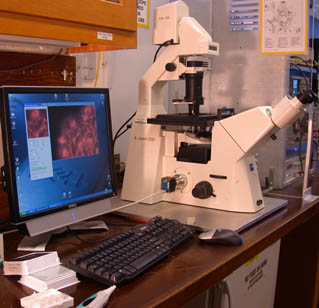
\includegraphics[width=\linewidth,keepaspectratio]{images/BMC_Station319.jpg}} \\
    \caption{The BMC Station}
\end{minipage}\hfill
\begin{minipage}{.49\linewidth}
    \href{http://experimentationlab.berkeley.edu/sites/default/files/images/Setup2.jpg}{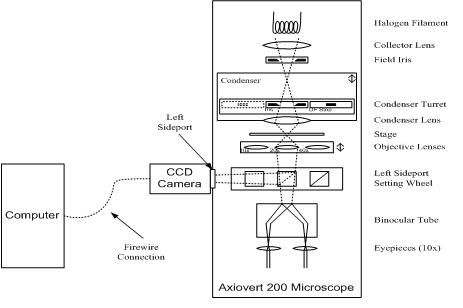
\includegraphics[width=\linewidth,keepaspectratio]{images/Setup2.jpg}} \\
    \caption{Block Diagram}
\end{minipage}
\end{figure}

You will prepare wet mount slides of polystyrene beads and onion epidermis peels to view on the light microscope pictured above (More specific explanations are found below). This is an inverted compound microscope, called inverted because the lenses are \emph{below} the stage, and the light source above. The microscope is outfitted with four objective lenses: 5x, 10x, 20x, and 40x. The most challenging technique you will learn is the proper adjustment of the condenser turret and iris diaphragms to achieve good bright-field Koehler illumination and dark-field illumination. It is worth learning this technique carefully, as it makes a big difference in the contrast and sharpness of your image. Aside from initial calibration and occasional high-power measurements, you will find the 20x objective and dark-field illumination most useful.

Once you have a specimen in good view through the eyepieces of the microscope, you'll use the CCD camera on the left side to transfer images to the computer. The particle tracker software will let you see a small part of the field of view of the microscope, and process movies live to identify particles and track them. Once you have fine tuned the microscope settings and software settings to get the software to track interesting particles and ignore artifacts and non-moving ones, you can start saving data to the hard drive. A dataset will consist of a set of x- and y-positions of a particle in each frame captured (at about 20 frames per second), for as many particles as were found. You can get diffusion coefficients from the software also, but keep in mind they are only valid for particles experiencing Brownian motion without any bulk flow.

\subsection{Experiment Timeline}

\subsubsection{By the end of your first day in the lab}

\begin{enumerate}
    \item Create a directory on the C drive of the Brownian motion experiment computer with your names (e.g. C:\textbackslash  JohnDoe\_JaneDoe). Copy the folder \textbf{C:\textbackslash  BMC\_Code }to your Directory you just created.  U: drive, 111 Lab Share, also has a copy of this folder. It is located at ``U:\textbackslash  Advanced Lab Share\textbackslash  Experiment Folders\textbackslash  BMC'' Remember to save a copy and all your data to ``My Documents'' or your ``Desktop'' each day to ensure it is backed up and so it will be available on any other computer you log onto in the 111-Lab.

    To execute the software go to --$>$
    
    \textbf{C:\textbackslash  BMC\_Code\textbackslash  Brownian Motion Software\textbackslash  BMC Code \\
    Student Version\textbackslash  BrownianApplication\textbackslash  bin\textbackslash  Debug\textbackslash  BrownianApplication.exe}
    
    Then click on the \textbf{Control Window}; then \textbf{Camera Go}; to exit program, \textbf{X} out the Control Window and all windows should close.
    
    \item Learn how to simulate and analyze Brownian motion of single particles using Matlab. Carry out the \href{http://experimentationlab.berkeley.edu/node/83}{\textbf{Simulating Brownian Motion}} exercise by copying Matlab code from the wiki page and pasting it into the Command Window in Matlab to generate the plots and analysis shown.
    
    \item After you understand how the Brownian-motion simulation works, adjust the parameters of the simulation to reflect the actual experimental conditions you chose above to generate simulated data that will be useful predictions to compare with your results.
\end{enumerate}

\subsubsection{By the end of your second day in the lab}

\begin{enumerate}
    \setcounter{enumi}{3}
    \item Complete the \hyperref[sec:CalibrationAndTesting]{Calibration and Testing} section of the lab to work out all of the techniques you will need.

    \item Complete the Improving the Particle Tracker section of the lab.
    
    \item Start on  \hyperref[sec:InvestigationI]{Investigation I}.
    
    \item Get your Mid-Lab \href{http://experimentationlab.berkeley.edu/BMCPreLab}{\textbf{BMC Pre Lab and Evaluation}} signed off. This should be the end of day 2.
\end{enumerate}

\subsubsection{By the end of days 3 - 4}

\begin{enumerate}
    \setcounter{enumi}{7}
    \item Complete your first investigation, \hyperref[sec:InvestigationI]{Effect of particle size and fluid properties on Brownian motion}.

    \item Make a slide of onion epidermal cells and conduct some preliminary observations. Decide on the research questions you want to investigate and write down your plan for the project.
\end{enumerate}

\subsubsection{By the end of days 5 - 6}

\begin{enumerate}
    \setcounter{enumi}{9}
    \item Complete your investigation of \hyperref[sec:InvestigationII]{Intracellular Movement in Onion Cells}.
\end{enumerate}

\subsubsection{After day 6}

\begin{enumerate}
    \setcounter{enumi}{10}
    \item Analyze your data.
\end{enumerate}

\section{Calibration and Testing}
\label{sec:CalibrationAndTesting}

Before taking data in your first investigation, you must calibrate the microscope and learn the experimental techniques involving pipetting, microscopy, and data-taking.

Your first slide preparation of 10 $\mu m$ beads will be used to determine the conversion from pixels in the image to $\mu$m on the actual specimen. This calibration must be done separately for the microscope's 20x objective lens and 40x objective lens. For the remainder of the lab, you will enter the appropriate conversion factor from pixels to $\mu m$ into the control panel of the particle tracker software in order for position data and statistics to be properly scaled.

For testing purposes, you will make a slide of 1 $\mu m$ beads in water, set up dark-field illumination on the microscope, and experiment with settings of the lighting, focus, and particle tracker software to successfully track beads and save data on particle motion. Setting up bright-field Kohler illumination and dark-field illumination requires careful alignment and some practice, but this will pay off later in the quality of your images and data.

\textbf{This is a checkpoint. Make sure you and your partner have the answer to Mid-lab part 1 question 2 before calling over a GSI or professor to sign you off.}

To perform the Calibration and Testing part of this lab, follow the instructions provide on the \href{http://experimentationlab.berkeley.edu/node/84}{\textbf{Experimental Procedures}} page.

\section{Investigation I. Effect of particle size and fluid properties on Brownian motion}
\label{sec:InvestigationI}

\subsection{Developing your Experiment}

This section is devoted to improving your experimental setup. The things listed below will improve your data collection but are not needed for all the data that you collect. Feel free to intersperse them with data-taking if you become frustrated.

\subsubsection{Choosing good experimental conditions}

There are three experimental parameters that you can control: the diameter of the test particles (the particles that will experience Brownian motion and be knocked around in the solution), the molecule that will provide the viscous solution (the solute), and the viscosity of the solution. We will assume temperature remains constant so it will not be one of the parameters.

To properly test Einstein's relation you should test at least three different viscosities. We suggest that for most of the experiment you use a particle size between 0.44 $\mu$m and 2 $\mu$m. If you go as small as 100nm, particles become difficult to detect (though still possible with good alignment of the optics), and at above 2 $\mu$m, they do not move around as much. To track large particles such as the 2 $\mu$m particles or larger, you will need to build the centroid algorithm discussed below to get sub-pixel accuracy.

To determine the effect of solvent molecule size on Brownian motion, you should run one of your experimental viscosity/particle size conditions with two different solvents -- one made of small solvent molecules (such as glycerol with a molecular weight of 92) and another with large molecules (such as polyvinylpyrollidone with an MW of 380,000). On the macro scale, the solutions you make up will have the same \emph{bulk viscosity} as measured, for example, by dropping a ball bearing through a column of the liquid. But the size and structure of the solute molecules may be important on the nanoscale. If somebody handed you a vial of 100 nm particles suspended in either PVP or glycerol, could you experimentally determine which solvent was used by looking at the Brownian motion?

Feel free to choose whatever experimental conditions you find interesting (explain why you chose them), but the recommended investigation is to try three different viscosities with one particle size and one solute, also one test with a much larger particle size (maybe 3.8 $\mu$m) and one test with a different solute (PVP or glycerol, whichever one you were not using before).

The microscope is an expensive and complicated piece of laboratory equipment. Before making any slides or viewing them in the microscope, read the \href{http://experimentationlab.berkeley.edu/node/84}{\textbf{Experimental Procedures}}.

\textbf{Checkpoint. Read Mid-Lab Questions Part 1 question numbers 3 and 4. When you have the answer / set up dark-field illumination, call over a GSI or professor to sign you off.}

\subsection{Analyzing Brownian Motion of Micro-Beads}

\subsubsection{Data Analysis: Brownian Motion}

In the first part of the data analysis, let's see if Einstein was right. Conceptually, the simplest thing to do is to sum over many particle trajectories to obtain a mean squared displacement, and to fit that directly to
\[
\left\langle {\left| \vec r(t+dt)-\vec r(t) \right|}^2 \right\rangle = 2 D dt
\]

Another method is described in \href{http://www.physics.nyu.edu/grierlab/methods/node11.html#eqes}{\textbf{Grier's particle tracking primer}}, their Eq. 16, and involves constructing a histogram of particle displacements for some fixed time interval, and then fitting this histogram to the expected Gaussian distribution. Of course, since you are using the same input data for both methods, your two estimates of \emph{D} should be comparable.

Now, calculate the value of the diffusion coefficient \emph{D} for each of the solutions and particle sizes you observed. Explain how you reached this value and what sources of error affected the result. How does your experimentally observed value differ from theoretical predictions? What factors does \emph{D} depend on?

Here are some follow up questions:

\begin{itemize}
    \item What relationship do you observe between viscosity, particle size, and diffusion coefficient?

    \item What is a Newtonian fluid?

    \item Are we really in the ``inertia-less'' regime? Why or why not?

    \item Can the exponential term in Langevin's general solution be neglected in your experiments? Why or why not?

    \item Imagine a particle diffusing not in an isotropic material, but in a mesh or network of some sort. Would it make sense to describe this process in terms of Einstein/Langevin diffusion?

    \item What would happen if your particles interacted through some potential?

    \item What is meant by viscous coupling? Is this something you need to take into account?

    \item Are your particle trajectories auto-correlated or cross-correlated? Over what timescales? What might lead to correlations?
\end{itemize}

\textbf{Checkpoint: Discuss a few of the previous questions with a GSI before moving on.}

\subsubsection{Optional Statistical Considerations: Correlations}

The starting point for our simulations was the assumption that we are in the over-damped limit, or the inertia-less regime. The benefit of this assumption is that we can generate trajectories very easily, by repeatedly querying a random number generator, and summing those displacements to find the overall trajectory. Of course, just because it's convenient doesn't mean it's true: do the particle trajectories you observed display any correlations? Our simulated trajectories should not, by construction.

How do we quantify possible correlations in a real or simulated particle trajectory? The concept of auto-correlation was invented to quantify the degree to which a particle's trajectory in the i'\emph{th} time interval depends on some preceding time interval. If you are familiar with Markov chains then these concepts will be second nature. The autocorrelation is defined as:
\begin{equation}
    \textrm{corr}(k) = \frac{\sum_{i=1}^N(x_i-\bar{x})*(x_{i+k}-\bar{x})}{\sum_{i=1}^N(x_i-\bar{x})^2}
\end{equation}
Unfortunately there are a very large number of different ways of implementing this function, depending on how rollover is handled and so forth. But mathematically, the expression is simple - leaving normalization aside, we have:
\begin{equation}
    \textrm{corr}(k) = \sum_{i=1}^N x_i*x_{i+k}
\end{equation}
which makes sense - the product of two identical numbers (corresponding to two perfectly correlated positions) will evaluate to a maximum. Subtracting the mean value, and dividing by $N \times$ variance, yields the correlation coefficient, a number that ranges from 1 (perfectly correlated) to 0 (uncorrelated). The concept of \href{http://physics111.lib.berkeley.edu/Physics111/Reprints/OTZ/biowikipedia.pdf}{\textbf{cross-correlation}} is an immediate extension of the concept of autocorrelation. There is a more practical discussion of computing the cross- and autocorrelation sequences in the last section of the \emph{Simulating Brownian Motion in Matlab }web pages.

In an ideal world, your experimental particle trajectories should not display any auto- or cross-correlations. In the real world, however, there are many different potential sources for such correlations.

\section{Investigation II. Intracellular Movement in Onion Cells}
\label{sec:InvestigationII}

We want to analyze intracellular transport within plant cells. Onions are ideal for this experiment due to their unique concentric-shelled structure. They have membranes in between each cell which are both resilient and made of a layer which is precisely one cell thick. This makes them both easy and beautiful to observe with a microscope.

Initially, you will be ignorant of both the viscosity and exact particle size. You will, however, be able to determine these quantities experimentally throughout the course of this experiment.

\subsection{Cellular Motion}

After observing the onion under proper optics you will quickly see that there is a lot of interesting activity. The particles exhibiting the most motion are generally called granules and may consist of either vesicles or \href{http://physics111.lib.berkeley.edu/Physics111/Reprints/OTZ/biowikipedia.pdf}{\textbf{mitochondria}}. You should see at least two types of motion inside the cell: namely, Brownian motion and active transport. Active transport can consist of motion along tightly defined paths in which a single particle is being transported, or it can consist of cytoplasmic streaming in which a large number of particles flow behind a large moving object such as an organelle.

You should make an effort to describe, both quantitatively and qualitatively, all of these modes of transport. The questions below are intended to get you thinking about the investigation and help you plan on what you are going to analyze during the course of the investigation.

For (non-Brownian) active transport, a good thing to measure would be the velocity. You should note however that in this system the velocity can be quite complex.

\begin{itemize}
    \item How fast are particles moving?

    \item In which directions?

    \item How consistent are particles' velocities in a particular region?

    \item What does this say about how they are propelled?

    \item Do particles move consistently or do they change direction and speed?

    \item Do particles move uni-directionally or do they cross each other?

    \item Generally, what is the velocity distribution of directed particles, and what are the variables of this distribution?
\end{itemize}

In terms of qualitative structure it is important to ask where these particles are going and where they are coming from.

\begin{itemize}
    \item Do they seem to cluster somewhere?

    \item Do you see any pattern about their orientation relative to the cell?

    \item Is there net flow inwards or outwards? Vorticity?

    \item What is the structure of these cellular highways?
\end{itemize}

\textbf{Checkpoint: Discuss a few of the previous questions with a GSI to demonstrate your understanding.}

\subsection{Analysis: Intracellular Transport}

This is a rather open investigation in terms of the analysis portion. You can choose to conduct your investigation by answering the analysis questions in , or you can design you own investigation by choosing . Do not however take this as an excuse to do no work. You will be graded on the quality of your findings.

\begin{itemize}
    \item Last day of the experiment please fill out the \href{\ExperimentEvaluation}{\textbf{Experiment Evaluation}}

\end{itemize}

\subsubsection{Analysis Option A}

\textbf{Molecular motors}

\begin{itemize}
    \item What is their average velocity? How do the velocities due to active transport compare to the velocities you observed in your experiments involving Brownian Motion? (You may wish to plot a histogram of particle velocities you observe).

    \item What is the amount of work needed to transport a vesicle from the perimeter of the cell to the center? (You can calculate this quantity based on Stokes Law using the particle size and viscosity of the cytosol that you have already determined).

    \item Read through the literature to determine the amount of energy that is released when ATP is hydrolyzed to ADP. Compare this quantity to the amount of work needed to transport a vesicle from the perimeter of the cell to the center.

    \item Calculate the minimum number of myosin motors required to transport a vesicle from the perimeter of the cell to its center. (Each powerstroke consumes the energy involved in converting a single molecule of ATP to ADP, remember to correct for the \emph{efficiency} of the myosin motors).
\end{itemize}

\subsubsection{Analysis Option B}

Find some aspect of intracellular transport you find interesting. Write up a proposal containing what you wish to investigate and how you will conduct your investigation. Decide on some questions that you are going to answer.

When you are ready, show your proposal to your professor for approval and then begin to conduct your investigation.

\begin{itemize}
    \item Last day of the experiment please fill out the \href{\ExperimentEvaluation}{\textbf{Experiment Evaluation}}

\end{itemize}

\section{References}
\label{sec:References}

\begin{enumerate}
    \item M. Haw, ``\href{http://physics111.lib.berkeley.edu/Physics111/Reprints/BMC/Colloidal\%20Suspensions\%20-\%20Haw.pdf}{\textbf{Colloidal suspensions, Brownian motion, molecular reality: a short history}}'', J. Phys. Condens. Matter (2002). Optional reading, but very good. Some sections are really good like section 4 on the Theory of Brownian motion and section 5 on the Quantitative measures from Brownian motion.

    \item L. Faucheux and A. Libchaber, ``\href{http://physics111.lib.berkeley.edu/Physics111/Reprints/BMC/BMC\_Reprints/Faucheux-Libchaber-Confined\_Brownian\_Motion.pdf}{\textbf{Confined Brownian Motion}}'', Physical Review E 49, 5158–5163(1994). This paper is a must read and helps uncover the details of the underlying physics.

    \item D. Murphy, Fundamentals of Light Microscopy and Electronic Imaging, Wiley (2001). More than you ever wanted to know about microscopes. The sections on Koehler illumination (page 6) and dark-field microscopy (page 112) are particularly relevant.

    \item \href{http://www.microscopyu.com/}{\textbf{http://www.microscopyu.com/}}. If you are interested in microscopy, there is a wealth of information here.

    \item Yokota, E; Shimmen, T: ``\href{http://physics111.lib.berkeley.edu/Physics111/Reprints/BMC/Cytoplasmic_Streaming-Shimmen.pdf}{\textbf{Cytoplasmic Streaming in Plants}}'' \emph{Current Opinion in Cell Biology}, February 2004, pp. 68-72.

    \item Lodish, Berk, Zipursky, Matsudaira, Baltimore, and Darnell. ``\href{http://physics111.lib.berkeley.edu/Physics111/Reprints/BMC/BMC\_Reprints/MyosinActinMotor.htm}{\textbf{Myosin: The Actin Motor Protein}}'' \emph{Molecular Cell Biology} W. H. Freeman and Company. This is an introductory biology textbook, so gives a good overview, but may not be as authoritative as some of the primary sources listed here.

    \item D. H. Schott, R. N. Collins, A. Bretscher. ``\href{http://physics111.lib.berkeley.edu/Physics111/Reprints/BMC/BMC\_Reprints/SecretoryVesicle-Schott.pdf}{\textbf{Secretory vesicle transport velocity in living cells depends on the myosin-V lever arm length}}'' \emph{The Journal of Cell Biology}, Volume 156, Number 1, 2002 pp. 35–39.
    
    \item S. Sideman, A. Landesberg. ``\href{http://physics111.lib.berkeley.edu/Physics111/Reprints/BMC/BMC\_Reprints/BioenergeticsLandesberg.pdf}{\textbf{Bioenergetics - Conversion of Biochemical to Mechanical Energy in the Cardiac Muscle}}'' Springer Publishing. 2002 p. 59

    \item J. A. Spudich. ``\href{http://physics111.lib.berkeley.edu/Physics111/Reprints/BMC/BMC\_Reprints/MolecularMotrs372515a0.pdf}{\textbf{How molecular motors work}}'' \emph{Nature} Vol 372, 8 December 1994 pp. 515-518. Good overview, but details on myosin are limited to a few types that had been studied at that time. 

    \item J. Pokorný. ``\href{http://physics111.lib.berkeley.edu/Physics111/Reprints/BMC/BMC\_Reprints/Langevin\_On\_the\_Theory\_of\_Brownian\_Motion.pdf}{\textbf{Excitation of vibrations in microtubules in living cells}}'' \emph{Bioelectrochemistry} Vol 63 June 2004 pp. 321– 326

    \item M. Tominaga, H. Kojima, E. Yokota1, H. Orii1, R. Nakamori, E. Katayama, M. Anson, T. Shimmen, and K. Oiwa. ``\href{http://physics111.lib.berkeley.edu/Physics111/Reprints/BMC/BMC\_Reprints/HigherPlantMyosin7595042a.pdf}{\textbf{Higher plant myosin XI moves processively on actin with 35 nm steps at high velocity}}'' \emph{The European Molecular Biology Organization} Vol 22, 17 March 2003 pp. 1263-1272. 

    \item G. Jedd and J. Chua ``\href{http://physics111.lib.berkeley.edu/Physics111/Reprints/BMC/BMC\_Reprints/VisualPeroxisomes384.pdf}{\textbf{Visualization of peroxisomes in living plant cells reveals acto-myosin-dependent cytoplasmic streaming and peroxisome budding}}'' Plant Cell Physiology Vol. 43(4): pg. 384-392. 2002. Includes study of vesicle transport in Arabadopsis and onion epidermis. 

    \item Zeiss \href{http://physics111.lib.berkeley.edu/Physics111/Reprints/BMC/BMC\_Reprints/Basic-standard\_microscope.pdf}{\textbf{Basic Standard Microscope Manual}}

    \item Brown, Robert. ``\href{http://physics111.lib.berkeley.edu/Physics111/Reprints/BMC/BMC\_Reprints/Brown\_A\_brief\_account\_of\_microscopical\_observations.pdf}{\textbf{A Brief Account of Microscopal Observations}}''

    \item Bangs Laboratories, Inc. ``\href{http://physics111.lib.berkeley.edu/Physics111/Reprints/BMC/Colloid\%20Data\%20Sheets.pdf}{\textbf{Colloid Data Sheet}}''

    \item Lemons, Don S. and Anthony Gythiel. ``\href{http://physics111.lib.berkeley.edu/Physics111/Reprints/BMC/Langevin_On\%20the\%20Theory\%20of\%20Brownian\%20Motion.pdf}{\textbf{Paul Langevin's 1908 Paper ''On the Theory of Brownian Motion``}}'' Am. J. Phys., Vol. 65, 11, Nov 1997.

    \item Perrin, Jean. ``\href{http://physics111.lib.berkeley.edu/Physics111/Reprints/BMC/BMC\_Reprints/Perrin\_Experiment.pdf}{\textbf{Brownian Motion and Molecular Reality}}''

    \item System Overview of ``\href{http://physics111.lib.berkeley.edu/Physics111/Reprints/BMC/BMC\_Reprints/Systemoverview\_Axiovert\_200\_MAT\_46-0015\_e.pdf}{\textbf{Axiovert 200}}'' and additional info ``\href{http://physics111.lib.berkeley.edu/Physics111/Reprints/BMC/BMC\_Reprints/Zeiss-Microscope\_46-0015\_e.pdf}{\textbf{here}}''

    \item \href{http://physics111.lib.berkeley.edu/Physics111/Reprints/BMC/Zeiss-Microscope\_46-0015\_e.pdf}{\textbf{Axiolab}} A Reflected Light Microscope\href{http://physics111.lib.berkeley.edu/Physics111/Reprints/BMC/Zeiss-Microscope\_46-0015\_e.pdf}{\textbf{}}information

    \item \href{http://physics111.lib.berkeley.edu/Physics111/Reprints/BMC/b-40-022-43dmicroscopyaxiovert100135135m.pdf}{\textbf{3D Microscopy}} for Axiovert 100/135/135 M Microscopes

    \item \href{http://physics111.lib.berkeley.edu/Physics111/Reprints/BMC/BMC\_Reprints/g-42-513-axiovert100.pdf}{\textbf{Operating Instructions}} for Axiovert 100/135/135 M Microscopes

    \item \href{http://physics111.lib.berkeley.edu/Physics111/Reprints/BMC/BMC\_Reprints/microscope-illuminator100-g-41-310.pdf}{\textbf{Microscope Illuminator 100}} Operating Instructions
\end{enumerate}

Other reprints and reference materials can be found on the \href{http://physics111.lib.berkeley.edu/Physics111/Reprints/BMC/BMC\_index.html}{\textbf{Physics 111 Library Site}}

\end{document}
